
\subsection{Wesentliche Begriffe}
\subsubsection{Beleihungsauslauf}
Der Beleihungsauslauf, auch als Loan-to-Value-Ratio bekannt, ist eine zentrale Kennzahl in der Immobilienfinanzierung \parencite{BelWertV_3}. Er wird definiert als:
\begin{equation}
    \text{Beleihungsauslauf} = \frac{\text{Darlehensbetrag}}{\text{Beleihungswert}}
    \label{eq:ltv}
\end{equation}

\noindent wobei:
\begin{itemize}
    \item Der Darlehensbetrag ist die Höhe des Darlehens.
    \item Der Beleihungswert ist der langfristig erzielbare Wert einer Immobilie, unabhängig von kurzfristigen Marktschwankungen.
\end{itemize}

Ein geringerer Beleihungsauslauf zeigt dem Kreditgeber ein reduziertes Risiko für Zahlungsausfälle an. Daraus ergibt sich ein erhöhter Beleihungsauslauf, was zu einem höheren Risiko führt und in der Regel zu weniger günstigen Bedingungen für den Kreditnehmer führt.

Um das Konzept zu verdeutlichen, wird ein Fallbeispiel einer Immobilienfinanzierung betrachtet: Ein Gutachter schätzt den Beleihungswert einer Immobilie auf 500.000 Euro.Die Person, die das Haus kaufen möchte, beantragt ein Darlehen in Höhe von 275.000 Euro. Die Person, die das Haus kaufen möchte, beantragt ein Darlehen von 275.000 Euro.
Der Beleihungsauslauf wird gemäß Gleichung \ref{eq:ltv} folgendermaßen berechnet:
\begin{equation}
    \text{Beleihungsauslauf} = \frac{\text{Darlehensbetrag}}{\text{Beleihungswert}} = \frac{275.000 \mbox{\texteuro}}{500.000 \mbox{\texteuro}} = 0,55 = 55\%
\end{equation}
Der Beleihungsauslauf in diesem Fall beträgt 55\%. Das bedeutet, dass 55\% des Immobilienwertes wird von der Bank finanziert. Die restlichen 45\% müssen durch Eigenkapital oder oder andere Einnahmequellen abgedeckt werden.
\subsubsection{Transitionsrisiken}
Transitionsrisiken bezeichnen das Risiko finanzieller Verluste für Institutionen, die aus dem Anpassungsprozess hin zu einer Wirtschaft mit weniger CO2-Emissionen und einer umweltfreundlicheren Ökonomie entstehen \parencite{ecb2020climate}. Dieses Konzept, das in den Bereichen ESG, Klimawandel, Wirtschaft und Finanzen breite Anwendung findet, umfasst vier Hauptkategorien: Technologie-, Marktpreis-, Regulierungs- und Reputationsrisiken.

Besonders exponiert gegenüber diesen Risiken ist der Immobiliensektor, der für etwa 40\% der globalen Treibhausgasemissionen verantwortlich zeichnet \parencite{unepfi2023realestate} und somit vor erheblichen Anpassungsherausforderungen steht.
Für diesen Sektorentstehen Transitionsrisiken vorwiegend durch regulatorische Änderungen, insbesondere durch neue Gesetze zu Energiepreisen und CO2-Steuern. Diese Entwicklungen zwingen den Sektor zu weitreichenden Anpassungen, um wettbewerbsfähig zu bleiben und gleichzeitig Nachhaltigkeitsziele zu erreichen.
\subsubsection{Physische Risiken}
Unter physischen Risiken versteht man Gefahren, die aus natürlichen Ereignissen oder Umweltbedingungen entstehen und negative Konsequenzen für Gesellschaft, Wirtschaft und Ökosysteme nach sich ziehen können \parencite{greenvisionsolutions_transitorische_2024}. Diese Risiken werden typischerweise in akute Risiken, die durch plötzliche extreme Ereignisse wie Überschwemmungen oder Stürme hervorgerufen werden, und chronische Risiken, die sich aus langfristigen klimatischen Veränderungen wie dem Meeresspiegelanstieg, Wasserstress, Biodiversitätsverlust und Ressourcenknappheit ergeben, unterteilt \parencite{dnb2019values}.

\subsubsection{Klimaszenarien des NGFS}
Das \ac{NGFS} hat 72 verschiedene Klimaszenarien entwickelt, wovon sechs für diese Arbeit ausgewählt wurden. Diese sechs Szenarien repräsentieren ein breites Spektrum möglicher Entwicklungen unter Berücksichtigung verschiedener physischer Risiken und Transitionsrisiken. In Abbildung \ref{fig:ngfs} ist die Darstellung der sechs Haupt-Szenarien des NGFS im Rahmenwerk zu sehen. In Tabelle \ref{tab:ngfs-framework} sind ausführliche Erläuterungen zu diesen Situationen enthalten.

\begin{figure}[htbp]
    \centering
    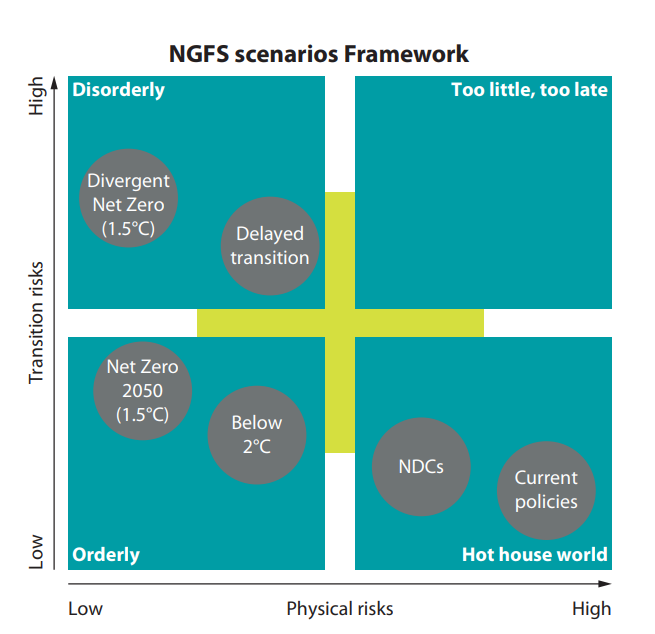
\includegraphics[width=0.7\textwidth]{figures/NGFS.png}
    \caption{NGFS Klimaszenario-Framework. Quelle: NGFS Climate Scenarios for central banks and supervisors (June 2021)}
    \label{fig:ngfs}
\end{figure}
\FloatBarrier

\begin{table}[htbp]
    \centering
    \small
    \caption{Überblick über NGFS-Rahmen zur Klassifizierung von Klimarisiken. In Anlehnung an Quelle: NGFS Climate Scenarios for central banks and supervisors (June 2021).}
    \label{tab:ngfs-framework}
    \begin{tabularx}{1.0\textwidth}{>{\raggedright\arraybackslash}X >{\centering\arraybackslash}X >{\centering\arraybackslash}X >{\raggedright\arraybackslash}X}
        \toprule
        \textbf{Szenario} & \textbf{Transitionsrisiken} & \textbf{Physische Risiken} & \textbf{Beschreibung} \\
        \midrule
        Orderly & Niedrig & Niedrig & Frühzeitige Einführung von Klimapolitiken, die allmählich strenger werden. Keine wesentlichen Diskrepanzen zwischen Politiken. \\
        \addlinespace
        Disorderly & Hoch & Niedrig & Höhere Transitionsrisiken aufgrund verzögerter oder inkonsistenter Klimapolitiken. Sehr strenge Politiken bei Einführung. \\
        \addlinespace
        Hot house world & Niedrig & Hoch & Nur wenige Länder führen Klimapolitiken ein. Globale Bemühungen unzureichend, führt zu irreversiblen Auswirkungen. \\
        \addlinespace
        Too little, too late & Hoch & Hoch & Extremste Szenarien. Unzureichende Maßnahmen führen zu Katastrophen und erzwingen einen ungeordneten Übergang. \\
        \bottomrule
    \end{tabularx}
\end{table}
\FloatBarrier

Die Szenarien "`Orderly"', "`Disorderly"' und "`Hot House World"' für die Jahre 2030, 2040 und 2050 stehen im Mittelpunkt. Im EZB-Klimarisiko-Stresstest werden sie mittels eines Bottom-up-Ansatzes berücksichtigt und beinhalten sowohl Transitions- als auch physische
Risiken. Diese Szenarien bilden die Grundlage für die Analyse der potenziellen Auswirkungen verschiedener Klimapolitiken auf den Immobiliensektor über einen längeren Zeitraum und ermöglichen eine detaillierte Untersuchung der Bruttowertschöpfung in diesem Sektor.

\subsubsection{Abflussmenge bei Hochwasser}\label{sec:HQ}

Die Festlegung von Hochwasserrisikogebieten in Deutschland erfolgt gesetzlich anhand der Anzahl von HQ\textsubscript{T\textsubscript{n} }-Ereignissen gemäß dem \textcite{WHG73}. Hierbei steht HQ für die Abflussmenge bei Hochwasser, während T\textsubscript{n} für den statistische Wiederkehrperiode des Ereignisses. Beispielsweise bezeichnet ein HQ\textsubscript{100} ein statistisch einmal in 100 Jahren auftretendes Hochwasserereignis.
In Bayern erfolgt eine detailliertere Klassifizierung von Hochwasserereignissen anhand ihrer statistischen Häufigkeit \autocite{BayLfU2019}:
\begin{itemize}
\item HQ\textsubscript{häufig}: Ein Hochwasser, das im Mittel alle 5 bis 20 Jahre auftritt und als "häufiges Hochwasser" bezeichnet wird.
\item HQ\textsubscript{100}: Ein Ereignis, das statistisch einmal in 100 Jahren zu erwarten ist.
\item HQ\textsubscript{extrem}: Ein sehr seltenes Extremhochwasser, das zu deutlich höheren Wasserständen als ein HQ\textsubscript{100} führen kann.
\end{itemize}
Durch diese Einteilung ist es möglich, Hochwassergefahren genauer zu bewerten und die Entwicklung von Schutzmaßnahmen zu unterstützen.